The edge device processing pipeline presented in Figure \ref{fig:edges} illustrates a compact and efficient architecture designed specifically for CPU-based edge devices equipped with a single-core CPU operating at 3.5 GHz and limited memory capacity of 512 MB RAM. This streamlined approach optimally addresses the constraints of computational resources while performing real-time video analytics directly at the network edge.

The pipeline operates through several integrated components that work together to achieve efficient video processing:

\begin{figure}[htbp]
    \centering
    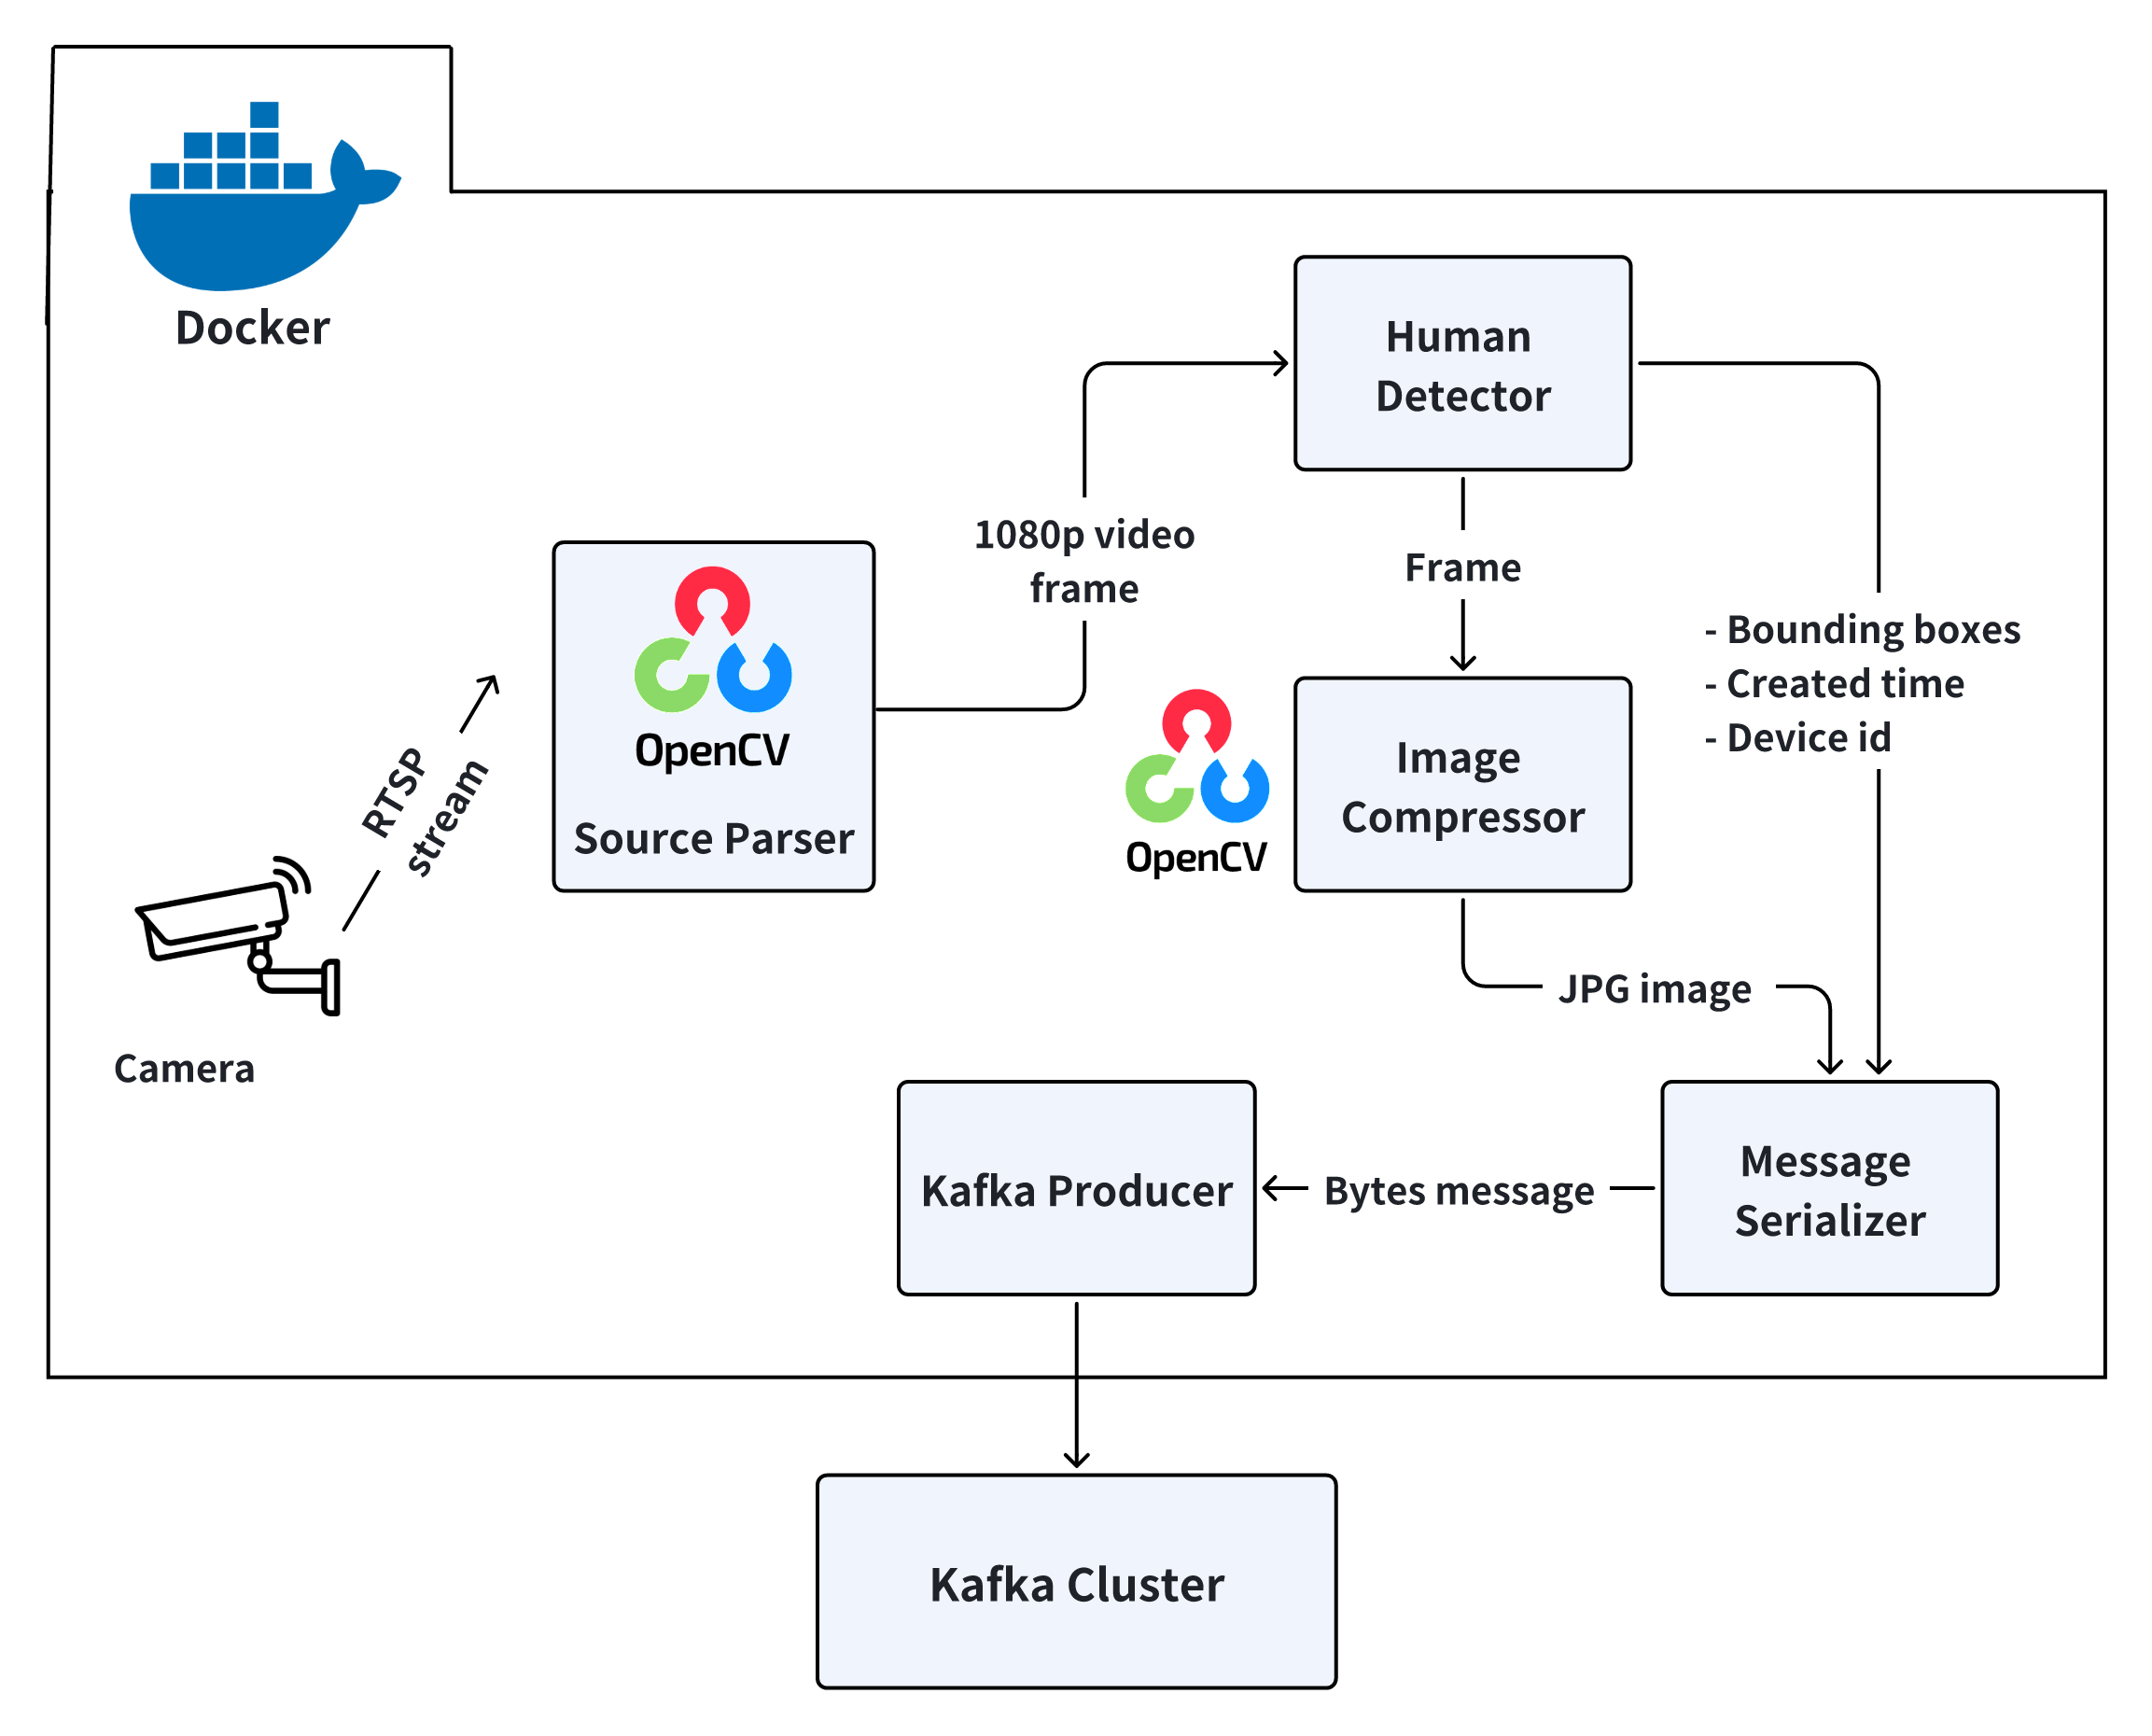
\includegraphics[width=1\textwidth]{Figure/edges.png}
    \caption{Edge devices processing pipeline}
    \label{fig:edges}
\end{figure}

\begin{itemize}
    \item \textit{Source parser}: This component handles input from RTSP cameras delivering live video streams or can be loaded from video sources. Both inputs are uniformly processed through an OpenCV-based source parser that standardizes the video streams into 1080p frames, thus simplifying subsequent processing steps and minimizing resource overhead.
    
    \item \textit{Human detector}: The standardized video frames are then processed by a lightweight yet robust YOLOv11 object detection model, excellently suited for human detection. This human detector module identifies human subjects within each frame, generating precise bounding box coordinates and essential metadata such as timestamp and device identifier.
    
    \item \textit{Image Compressor}: To further optimize resource usage, the original video frames undergo simultaneous compression using OpenCV's image processing capabilities, producing compressed JPG images. This significantly reduces the data size but still feasible for constrained CPU environments, without compromising analytical quality.
    
    \item \textit{Message Serializer}: Detection results along with the compressed images are efficiently structured into Avro schema serialized messages, significantly improving serialization speed and resource efficiency.
    
    \item \textit{Kafka producer}: Finally, these structured messages are published to Kafka \texttt{reid\_input} topic via Kafka producer framework, enabling asynchronous, real-time communication with centralized server without being blocked by the centralized server processing.
\end{itemize}

This targeted approach ensures minimal resource consumption, reduced network bandwidth requirements, prompt local analytics responses, and increased scalability by distributing the video processing workload across multiple constrained CPU-based edge devices.


\subsection{Human detector}
\label{sec:edge_human_detection}

As illustrated in Figure \ref{fig:edges}, human detector is the first component in the edge device processing pipeline, after receiving the output from source parser. It is responsible for detecting humans in the video frames and generating bounding box coordinates and essential metadata such as timestamp and device identifier.

The YOLOv11n model deployed within the edge device processing pipeline serves as a robust and resource-efficient solution for real-time human detection, optimized specifically for environments with constrained computational resources.

\subsubsection{Inference configuration}

The inference setup for YOLOv11n is carefully optimized to balance accuracy and computational efficiency, particularly suitable for CPU-based edge devices. Key configurations include:

\begin{itemize}
    \item \textit{Confidence Threshold:} \textbf{0.25}\\
    This threshold is specifically chosen to complement ByteTrack, a multi-object tracking algorithm used in the subsequent pipeline stage. ByteTrack effectively manages object disappearance by utilizing two stages of tracklet association: one for high-confidence tracklets and another for low-confidence tracklets. The confidence threshold of $0.25$ provides a balanced trade-off, ensuring objects are consistently tracked without introducing excessive noise from low-confidence detections.


    \item \textit{Class ID:} \textbf{0}\\
    Although YOLO is trained on large-scale datasets like COCO, containing 80 classes, our pipeline exclusively focuses on detecting humans. Hence, we restrict detection to class ID $0$, which corresponds specifically to humans,  improving efficiency and simplifying subsequent processing.

    \item \textit{Inference Device:} \textbf{CPU}\\
    The inference is conducted entirely on the CPU, aligning with the constrained computing resources typically available in edge deployment scenarios.s
\end{itemize}

Post-inference, only the following essential detection data are extracted for efficient downstream processing:

\begin{figure}[htbp]
    \centering
    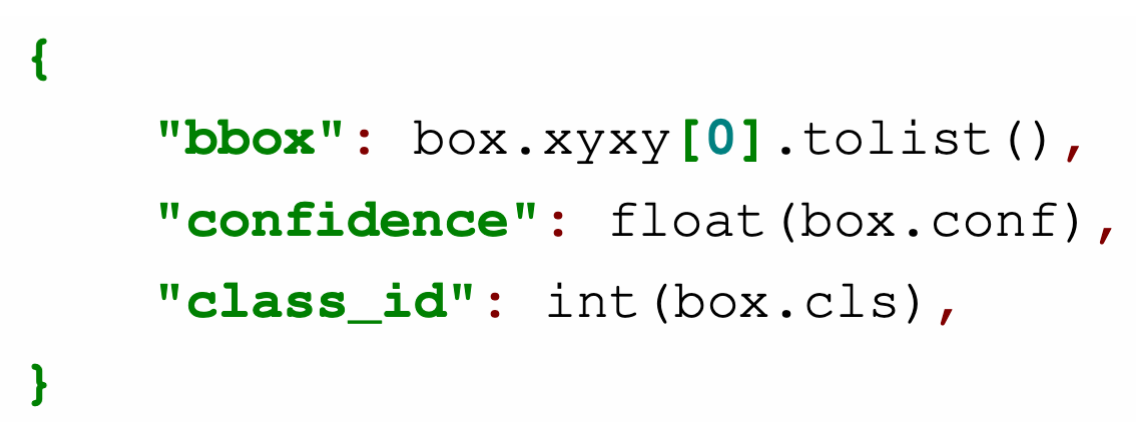
\includegraphics[width=0.7\textwidth]{Figure/bboxes_yolo.png}
    \caption{Extracted bounding box information after inference}
    \label{fig:bboxes_yolo}
\end{figure}

The bounding box information follows a structured format specifically designed for optimal performance:

\begin{itemize}
    \item \textbf{bbox}: Coordinates are extracted in xyxy format, representing the top-left corner $(x_1, y_1)$ and bottom-right corner $(x_2, y_2)$ of the detected human bounding box. This format is particularly efficient for subsequent tracking algorithms and provides direct compatibility with ByteTrack's input requirements.
    
    \item \textbf{confidence}: The detection confidence score is converted to a floating-point value ranging from 0.0 to 1.0, indicating the model's certainty about the presence of a human in the detected region. This score is crucial for the two-stage association process in ByteTrack.
    
    \item \textbf{class\_id}: Since the system focuses exclusively on human detection, this field consistently contains the value 0 (corresponding to the "person" class in COCO dataset). While redundant in single-class scenarios, maintaining this field ensures compatibility with multi-class detection pipelines and facilitates future system extensions.
\end{itemize}

This minimal yet comprehensive data structure ensures that only essential information is transmitted to the Kafka cluster, significantly reducing message payload size while preserving all necessary data for accurate tracking and Re-ID processing at the centralized server.



\subsubsection{Introducing to ONNX model format}

For further optimization, YOLOv11 is converted from the PyTorch (\texttt{.pt}) format to ONNX (Open Neural Network Exchange), enabling interoperability and improved inference performance in CPU-based deployment environments. The ONNX format facilitates dynamic and simplified computation graphs, significantly enhancing processing efficiency and reducing latency during real-time detection tasks on the edge device.

The conversion process is automated, utilizing YOLO's built-in export function that dynamically simplifies the computation graph to maintain a lightweight and efficient model suitable for low-resource environments:

\begin{figure}[htbp]
    \centering
    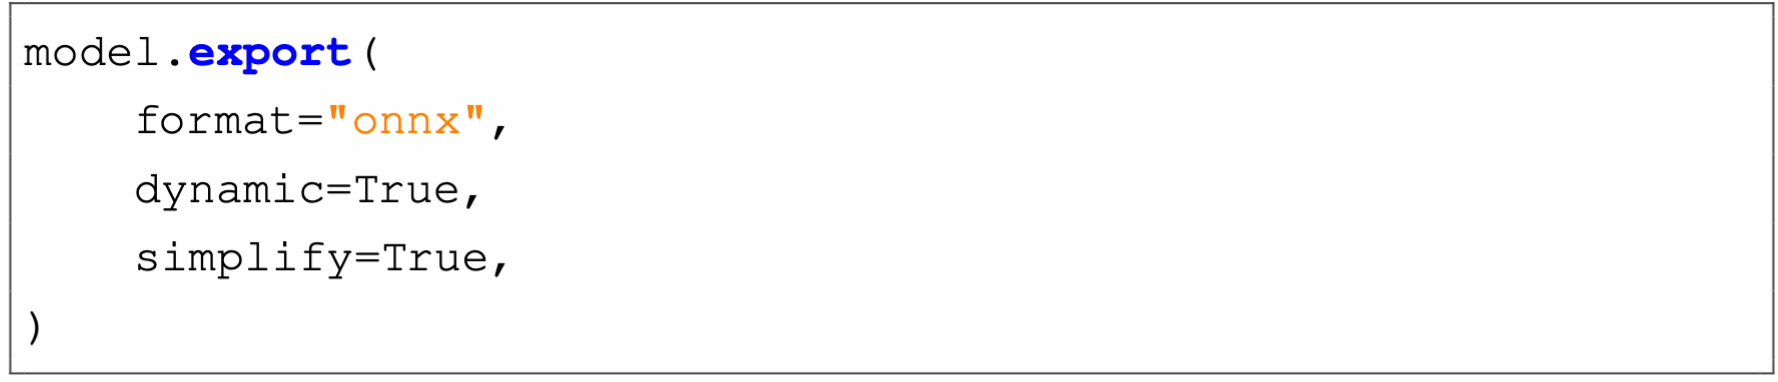
\includegraphics[width=1\textwidth]{Figure/onnx_command.png}
    \caption{ONNX model conversion command}
    \label{fig:onnx_command}
\end{figure}

Here, the \texttt{dynamic=True} flag ensures that the model can handle varying input sizes, while the \texttt{simplify=True} flag simplifies the model to reduce unnecessary operations, resulting in a more efficient and streamlined model. The output ONNX model is saved in the \texttt{yolo11n.onnx} file.


\subsubsection{Introducing to OpenVINO model format}

Alternatively, for Intel hardware-based edge deployments, YOLOv11 is converted into the OpenVINO model format. This conversion leverages Intel's OpenVINO toolkit, which provides further optimizations tailored specifically for CPU inference on Intel architectures. OpenVINO models offer reduced inference time and enhanced resource utilization, ensuring optimal performance within the specified hardware constraints of single-core CPUs and limited RAM.

The OpenVINO conversion is similarly automated using YOLO's export utilities, producing optimized models capable of handling real-time analytics tasks efficiently under the given hardware limitations:

\begin{figure}[htbp]
    \centering
    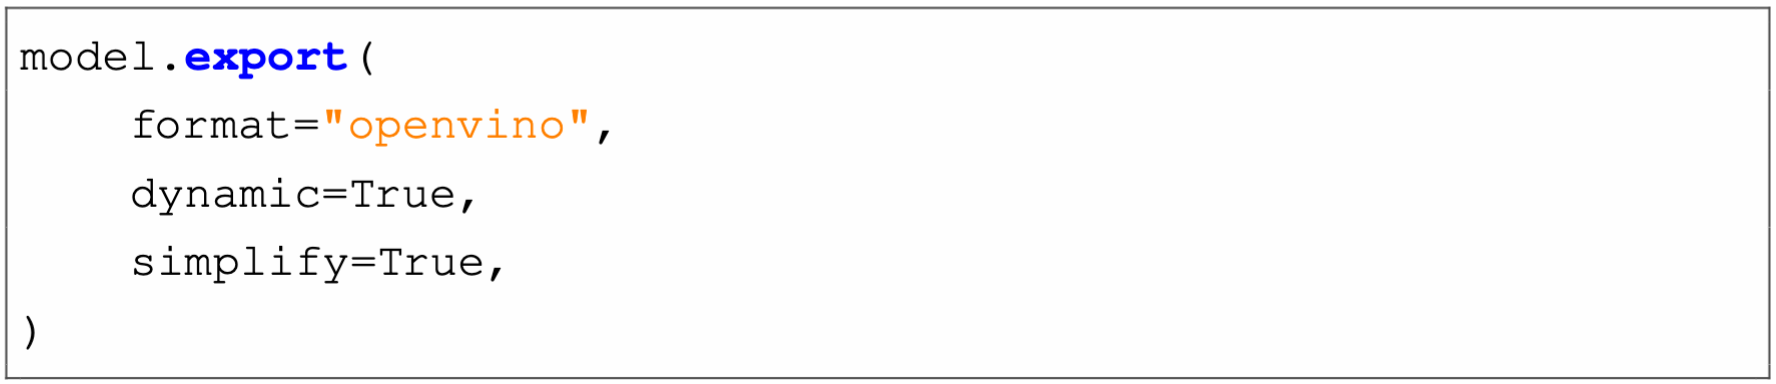
\includegraphics[width=1\textwidth]{Figure/openvino_command.png}
    \caption{OpenVINO model conversion command}
    \label{fig:openvino_command}
\end{figure}

Similar to the ONNX conversion, the \texttt{dynamic=True} flag ensures that the model can handle varying input sizes, while the \texttt{simplify=True} flag simplifies the model to reduce unnecessary operations, resulting in a more efficient and streamlined model. The output OpenVINO model is saved inside a folder which contains 3 files:
\begin{itemize}
    \item \texttt{yolo11n.xml}
    \item \texttt{yolo11n.bin}
    \item \texttt{metadata.yaml}
\end{itemize}


To determine the optimal model format for edge deployment scenarios, a comprehensive comparative evaluation is conducted across multiple performance metrics in Section~\ref{sec:detection_experiments}. This evaluation systematically analyzes inference latency, memory consumption, CPU utilization, and detection accuracy across PyTorch (.pt), ONNX, and OpenVINO formats under the specified hardware constraints. The results provide empirical evidence to guide format selection based on specific deployment requirements and hardware configurations.


\subsection{Image compressor with OpenCV}
\label{sec:edge_image_compression}

As mentioned in Section \ref{sec:message_serialization}, the original video frames of FullHD resolution (1920x1080) have a size of around 2MB. If we keep the original image quality, the total message size would be too large for practical network bandwidth and storage. Therefore, there is a need to compress the image quality.

OpenCV provides a simple and effective way to compress the image quality by using the \texttt{cv2.imencode} function. The function takes a quality parameter which ranges from 0 to 100, where 0 is the highest compression and 100 is the original image quality.

\begin{lstlisting}[language=python, caption={Image compression with OpenCV}]
cv2.imencode(".jpg", frame, [cv2.IMWRITE_JPEG_QUALITY, 70])
\end{lstlisting}

The function \texttt{cv2.imencode} requires 3 main parameters:
\begin{itemize}
    \item \texttt{".jpg"}: The image format. Here, we use the JPEG format for efficient compression.
    \item \texttt{frame}: The image frame to be compressed in numpy array format.
    \item \texttt{IMWRITE\_JPEG\_QUALITY}: The quality parameter. Here, we set the quality to 70, which is a good balance between compression and image quality.
\end{itemize}

\begin{figure}[htbp]
    \centering
    \begin{subfigure}{0.45\textwidth}
        \centering
        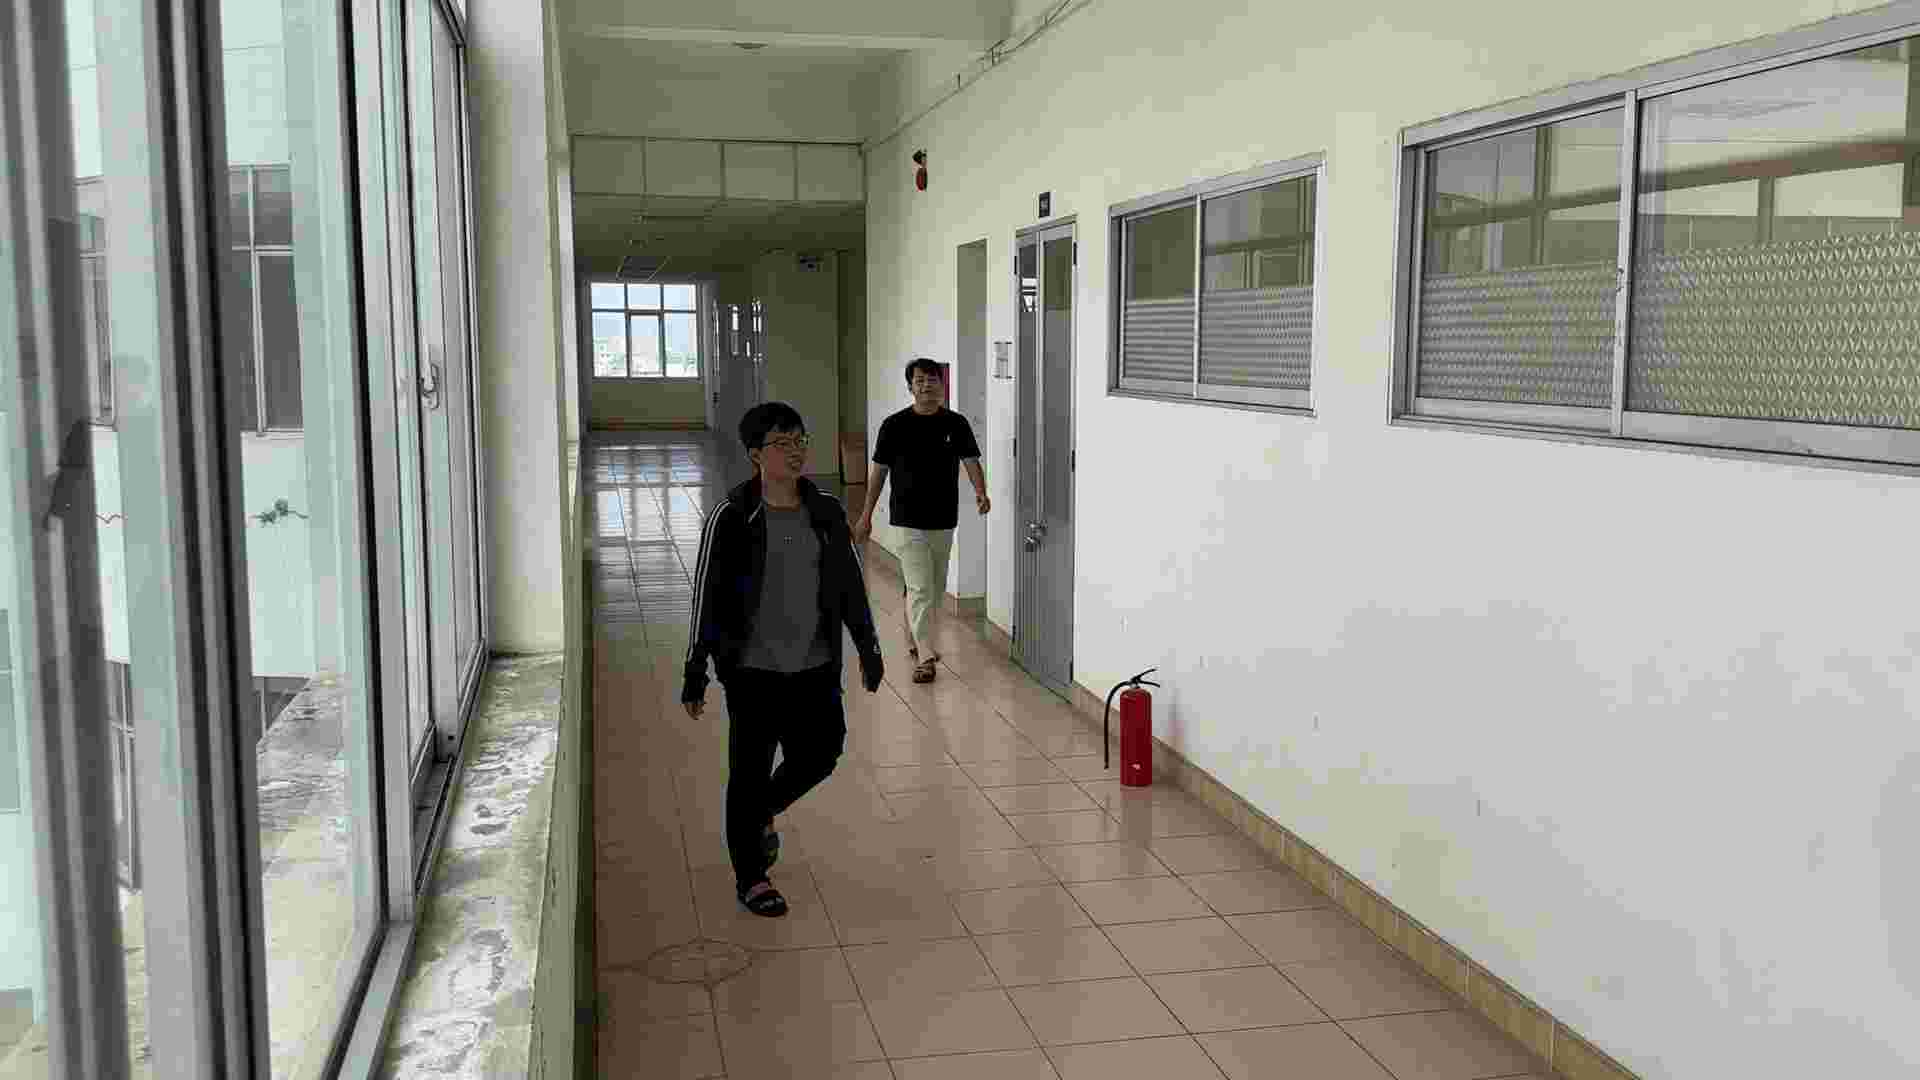
\includegraphics[width=\textwidth]{Figure/frame_0_quality_10.jpg}
        \caption{Quality 10 - 62KB}
        \label{fig:quality_10}
    \end{subfigure}
    \hfill
    \begin{subfigure}{0.45\textwidth}
        \centering
        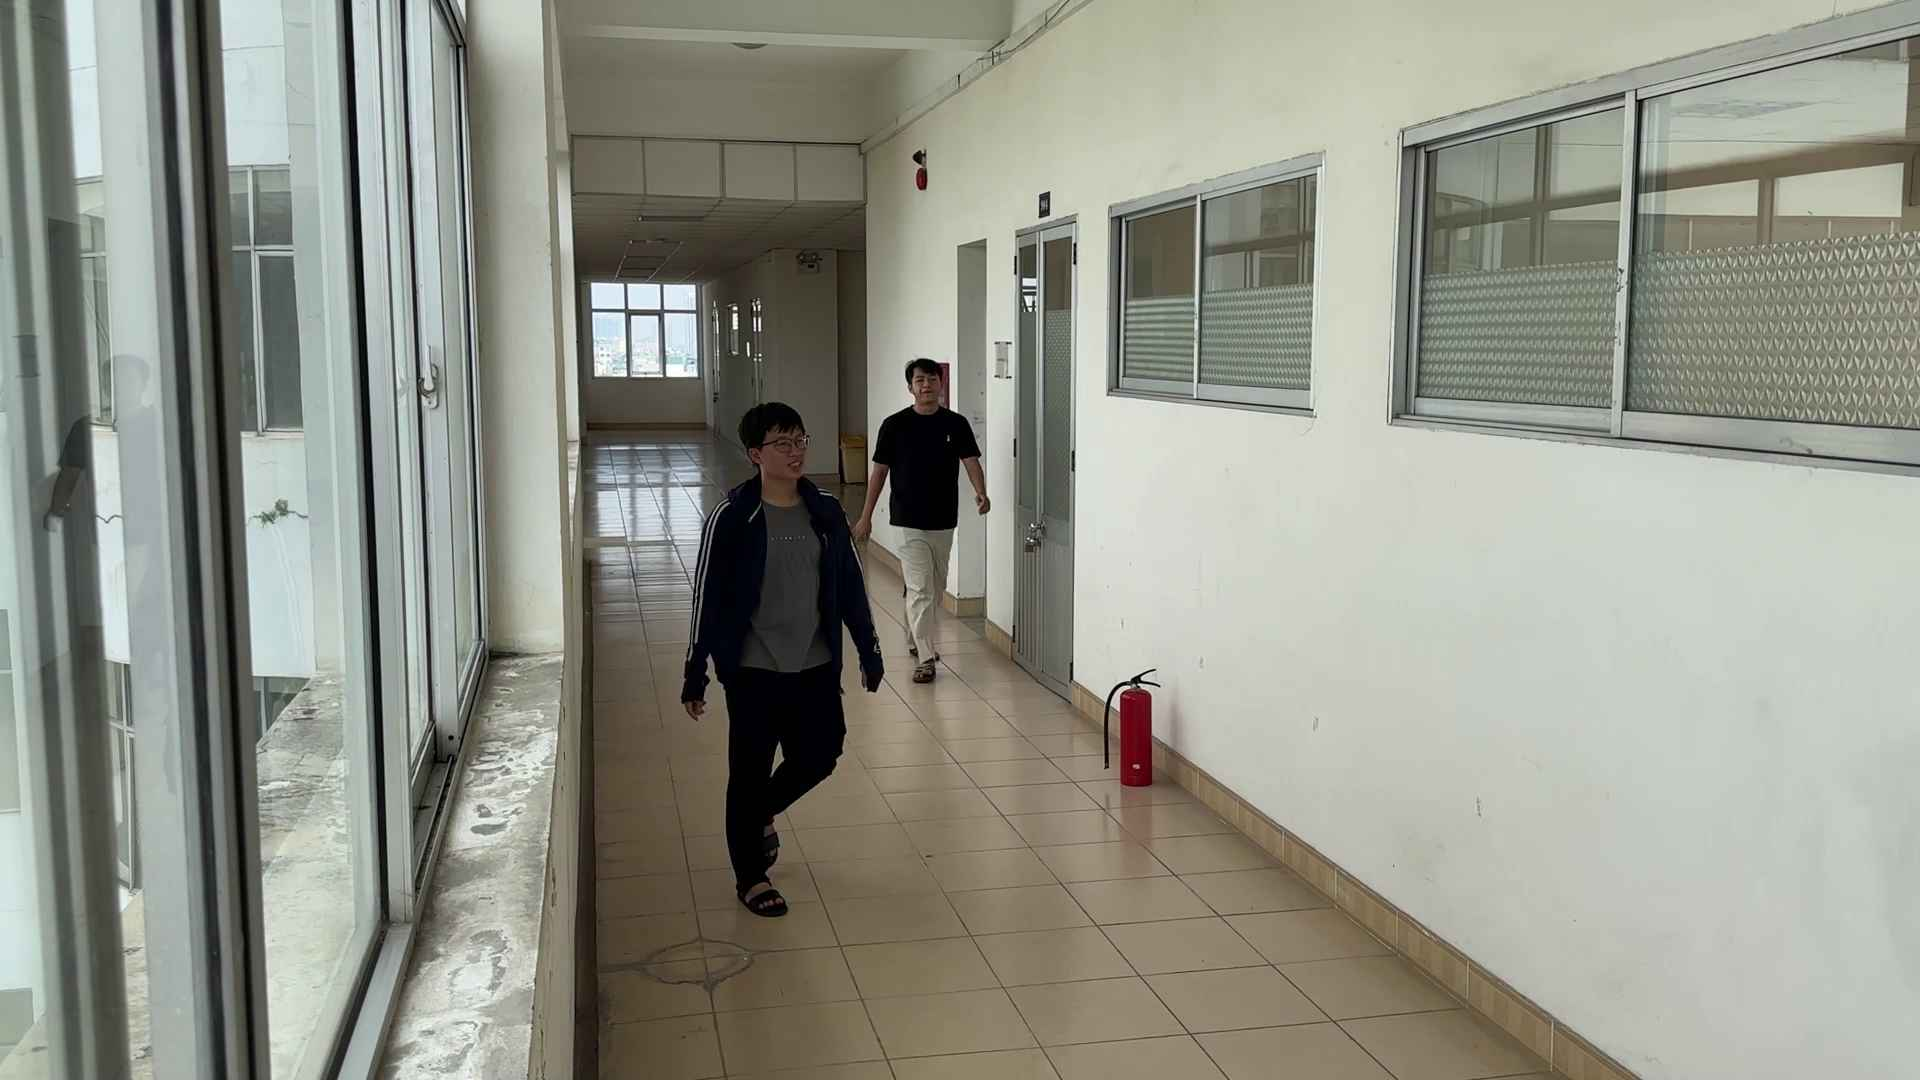
\includegraphics[width=\textwidth]{Figure/frame_0_quality_40.jpg}
        \caption{Quality 40 - 116KB}
        \label{fig:quality_40}
    \end{subfigure}
    
    \vspace{0.5cm}
    
    \begin{subfigure}{0.45\textwidth}
        \centering
        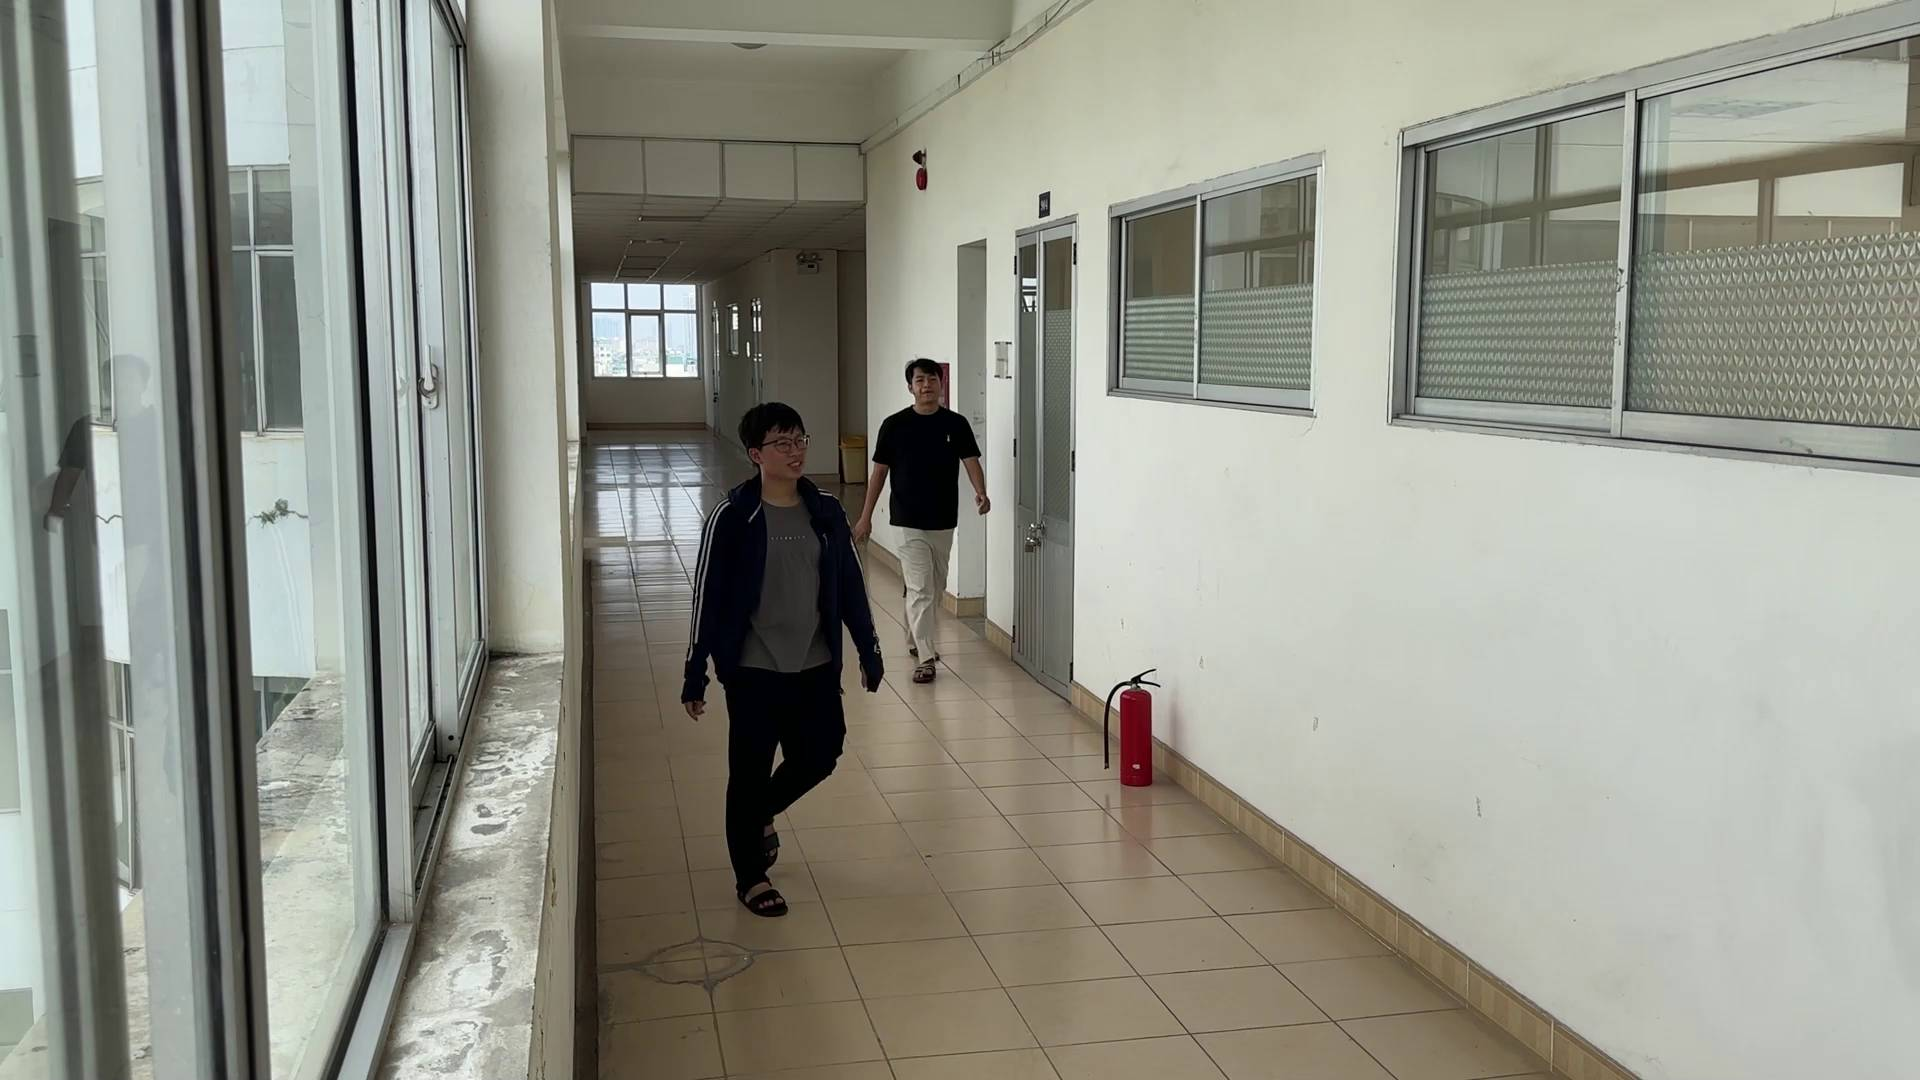
\includegraphics[width=\textwidth]{Figure/frame_0_quality_70.jpg}
        \caption{Quality 70 - 168KB}
        \label{fig:quality_70}
    \end{subfigure}
    \hfill
    \begin{subfigure}{0.45\textwidth}
        \centering
        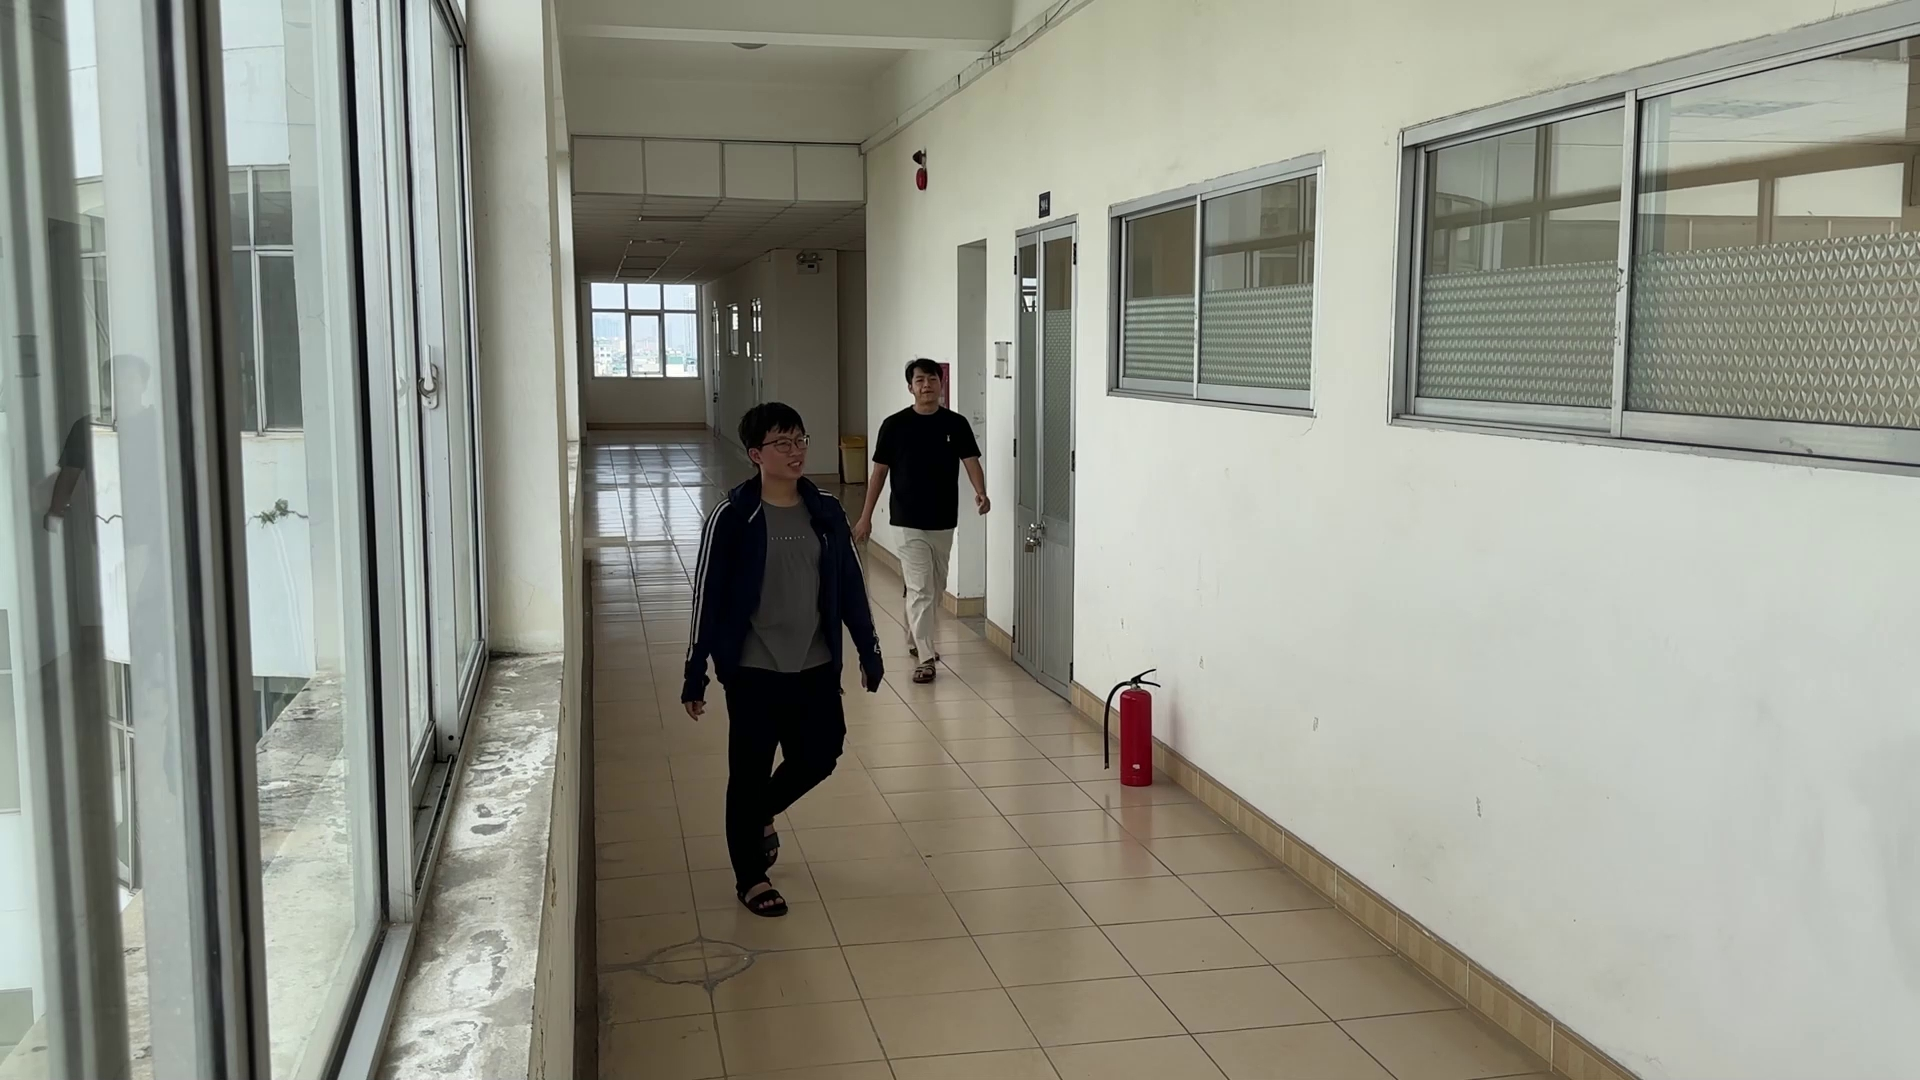
\includegraphics[width=\textwidth]{Figure/frame_0_quality_100.jpg}
        \caption{Quality 100 - 747KB}
        \label{fig:quality_100}
    \end{subfigure}
    
    \caption{Comparison of JPEG compression quality levels showing the trade-off between file size and image quality. Quality 10 provides maximum compression - only 62KB, but with noticeable quality loss, while quality 100 maintains original image quality with larger file size - 747KB. Quality of 70 provides a good balance between compression and image quality - 168KB.}
    \label{fig:jpeg_quality_comparison}
\end{figure}

\subsection{Messages serialization}
\label{sec:edge_message_serialization}

\begin{figure}[htbp]
    \centering
    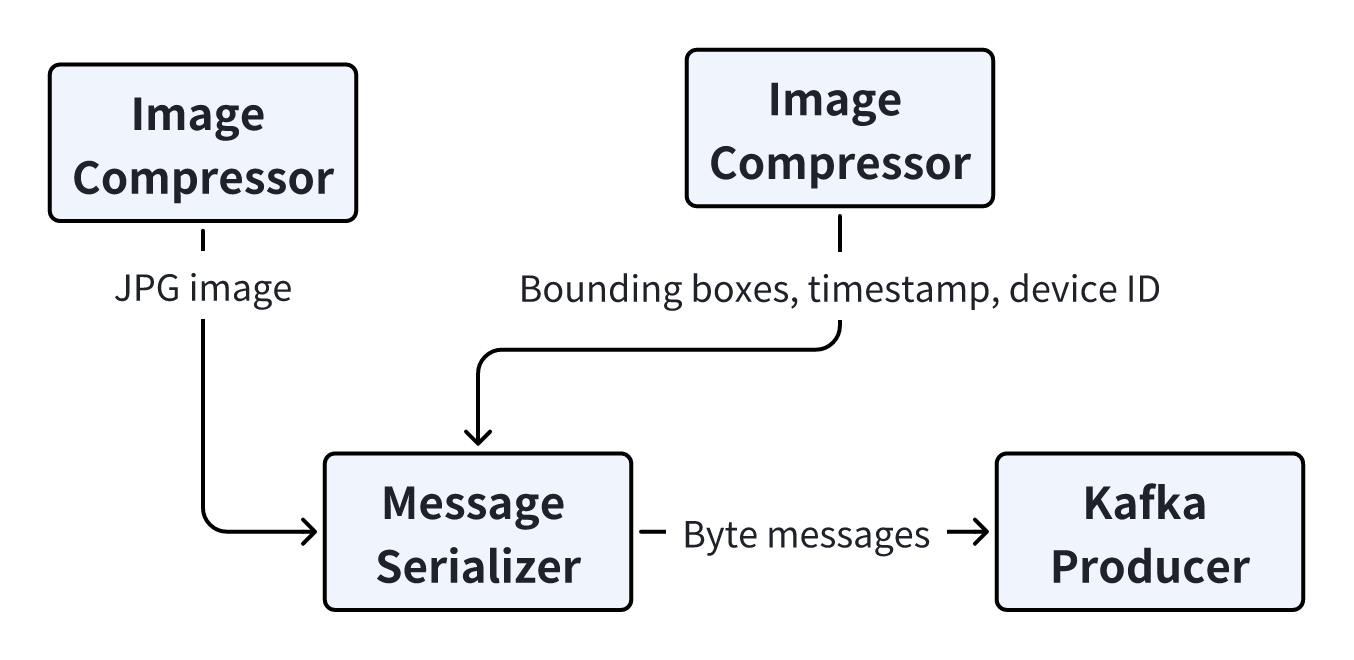
\includegraphics[width=0.7\textwidth]{Figure/edge_mess.png}
    \caption{Message serialization flow}
    \label{fig:edge_mess}
\end{figure}

As mentioned in Section \ref{sec:message_serialization}, the detection results along with the compressed images are structured into Avro schema serialized messages before being published to Kafka.

\begin{figure}[htbp]
    \centering
    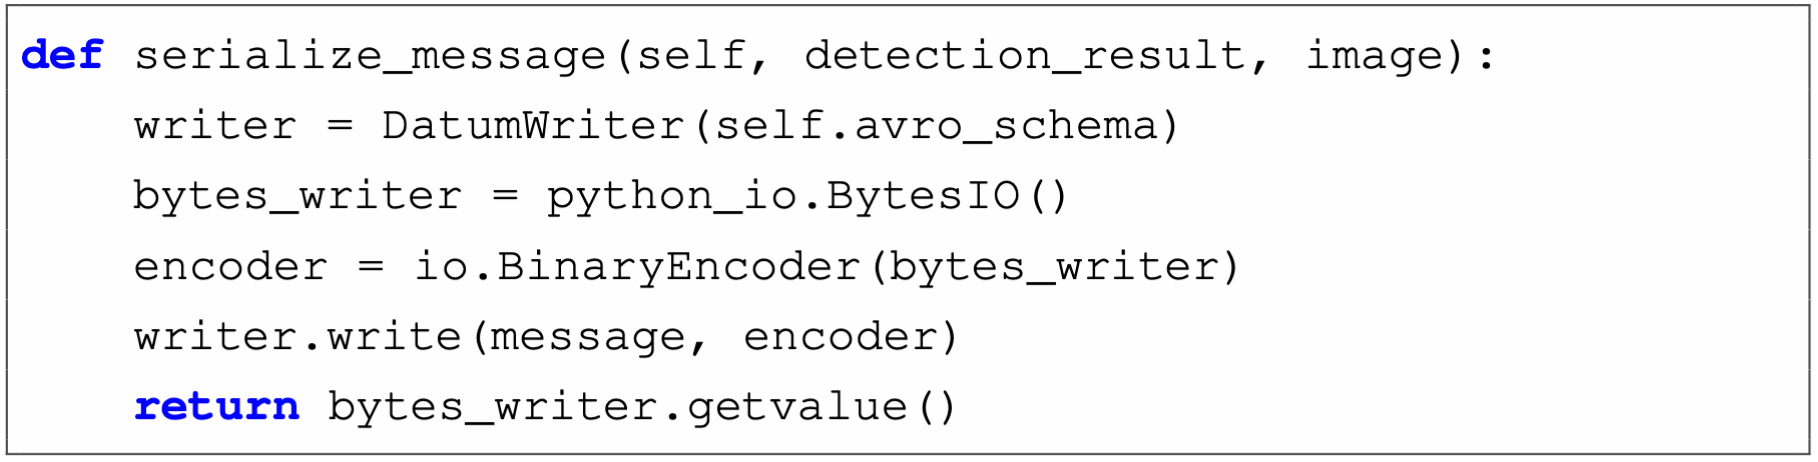
\includegraphics[width=1\textwidth]{Figure/avro_code.png}
    \caption{Message serialization with Avro schema, using \texttt{DatumWriter} and \texttt{BinaryEncoder}}
    \label{fig:avro_code}
\end{figure}

The \texttt{DatumWriter} class take the parsed the Avro schema and create a writer object. The \texttt{bytes\_writer} is a buffer to store the serialized message. The \texttt{encoder} is a binary encoder to encode the message. The \texttt{writer.write} method takes the message and the encoder, and write the message to the buffer. Finally, the \texttt{bytes\_writer.getvalue()} method returns the serialized message in bytes, before being published to Kafka cluster via \textbf{Kafka producer} framework.

\subsection{Containerization with Docker}
\label{sec:edge_containerization}

The edge device application is containerized using Docker to ensure consistent deployment across different hardware platforms and operating systems. The containerization strategy employs a multi-stage build approach that optimizes both build time and final image size, which are critical considerations for resource-constrained edge environments.

\subsubsection{Multi-stage build architecture}

The Docker configuration utilizes a two-stage build process designed to maximize efficiency and minimize the final container footprint. This approach addresses the specific constraints of edge computing environments where storage space and deployment speed are critical considerations.

\begin{lstlisting}[language=yaml, caption={Multi-stage Docker build configuration for edge deployment}]
# Build stage
FROM ghcr.io/astral-sh/uv:python3.11-bookworm-slim AS builder
ENV UV_COMPILE_BYTECODE=1 \
    UV_LINK_MODE=copy \
    UV_PYTHON_DOWNLOADS=0
WORKDIR /app
# Copy dependency files first for better caching
COPY pyproject.toml uv.lock ./
# Install dependencies in virtual environment
RUN uv sync --locked --no-dev
# Production stage
FROM python:3.11-slim-bookworm AS production
# Install system dependencies required for OpenCV
RUN apt-get update && apt-get install -y \
    libgl1-mesa-glx \
    libglib2.0-0 \
    libsm6 \
    libavcodec-dev \
    libavformat-dev \
    libswscale-dev \
    libjpeg-dev \
    && rm -rf /var/lib/apt/lists/*
WORKDIR /app
# Copy virtual environment from builder
COPY --from=builder /app/.venv /app/.venv
# Copy source code
COPY . .
# Set environment variables
ENV PATH="/app/.venv/bin:$PATH" \
    PYTHONPATH=/app \
    PYTHONUNBUFFERED=1
# Set the entrypoint to run main.py with arguments
ENTRYPOINT ["python", "-m", "src"]
\end{lstlisting}

\subsubsection{Build stage optimization}

The first stage, designated as the \textbf{builder} stage, leverages the specialized \texttt{uv} base image from Astral, which provides an ultra-fast Python package installer and resolver. This stage is specifically optimized for dependency management:

\begin{itemize}
    \item \textbf{Efficient dependency resolution}: The \texttt{uv} tool significantly reduces dependency installation time compared to traditional \texttt{pip}, which is particularly beneficial during development iterations when dependencies may change frequently.
    
    \item \textbf{Layer caching optimization}: By copying only \texttt{pyproject.toml} and \texttt{uv.lock} files first, Docker can effectively cache the dependency installation layer. This means that subsequent builds will only reinstall dependencies if these files change, dramatically reducing build times during development.
    
    \item \textbf{Bytecode compilation}: The \texttt{UV\_COMPILE\_BYTECODE=1} environment variable ensures that Python bytecode is compiled during the build process, improving runtime performance on edge devices where CPU resources are limited.
    
    \item \textbf{Production-only dependencies}: The \texttt{--no-dev} flag excludes development dependencies from the final build, reducing the virtual environment size and eliminating unnecessary packages that could introduce security vulnerabilities or consume valuable storage space.
\end{itemize}

\subsubsection{Production stage configuration}

The second stage creates the final production image with several key optimizations for edge deployment:

\begin{itemize}
    \item \textbf{Minimal base image}: The \texttt{python:3.11-slim-bookworm} base image provides the essential Python runtime while maintaining a small footprint, crucial for edge devices with limited storage capacity.
    
    \item \textbf{System dependencies}: Essential libraries for OpenCV and video processing are installed, including:
    \begin{itemize}
        \item \texttt{libgl1-mesa-glx}: OpenGL support for computer vision operations
        \item \texttt{libavcodec-dev}, \texttt{libavformat-dev}, \texttt{libswscale-dev}: FFmpeg libraries for video codec support
        \item \texttt{libjpeg-dev}: JPEG compression/decompression capabilities
    \end{itemize}
    
    \item \textbf{Virtual environment transfer}: The complete virtual environment is copied from the builder stage, ensuring all dependencies are properly isolated and configured without requiring reinstallation.
    
    \item \textbf{Runtime optimization}: Environment variables are configured to optimize Python execution:
    \begin{itemize}
        \item \texttt{PYTHONUNBUFFERED=1}: Ensures immediate output flushing for real-time logging
        \item \texttt{PYTHONPATH=/app}: Facilitates proper module resolution
    \end{itemize}
\end{itemize}

\subsubsection{Caching benefits and deployment efficiency}

This multi-stage approach provides several significant advantages for edge deployment scenarios:

\begin{itemize}
    \item \textbf{Reduced image size}: By excluding build tools and development dependencies from the final image, the production container is significantly smaller, reducing deployment time and storage requirements on edge devices.
    
    \item \textbf{Improved build caching}: Docker's layer caching mechanism ensures that dependency installation only occurs when \texttt{pyproject.toml} or \texttt{uv.lock} changes, dramatically reducing build times during iterative development from minutes to seconds.
    
    \item \textbf{Reproducible builds}: The locked dependency file (\texttt{uv.lock}) ensures identical dependency versions across all deployments, eliminating version conflicts and ensuring consistent behavior across different edge devices.
    
    \item \textbf{Security optimization}: The minimal production image reduces the attack surface by excluding unnecessary development tools and libraries, enhancing security for edge deployments in potentially untrusted environments.
    
    \item \textbf{Resource efficiency}: The optimized container consumes less memory and storage, allowing more efficient utilization of the limited resources available on edge devices while maintaining full functionality.
\end{itemize}

This containerization strategy ensures that the edge application can be consistently deployed across diverse hardware platforms while maintaining optimal performance within the specified constraints of single-core CPUs and 512 MB RAM limitations.

